
% ------------------------------------------------------------
% ------------------------------------------------------------

\section[Geo]{Geographical Plots}
%%%%%%%%%%%%%%%%%%%%%%%%%%%%%%%%%%%%%
\subsection{Maps}
%%%%%%%%%%%%%%%%%%%%%%%%%%%%%%%%%%%%%

\begin{frame}[fragile]
\frametitle{Geographic Maps}
  \framesubtitle{Map of Fiji Earthquakes Since 1964}

To overlay a map to a plot containing latitude and longitude, load the package \ttfamily maps: \normalfont 
    \begin{columns}
      \column{0.50\textwidth}
\begin{lstlisting}
data(quakes)
library(maps)
plot(quakes[, 2], quakes[, 1], xlim=c(100, 190), ylim=c(-40, 0))
map("world", add=T)
\end{lstlisting}

     \column{0.50\textwidth}
       \begin{center}
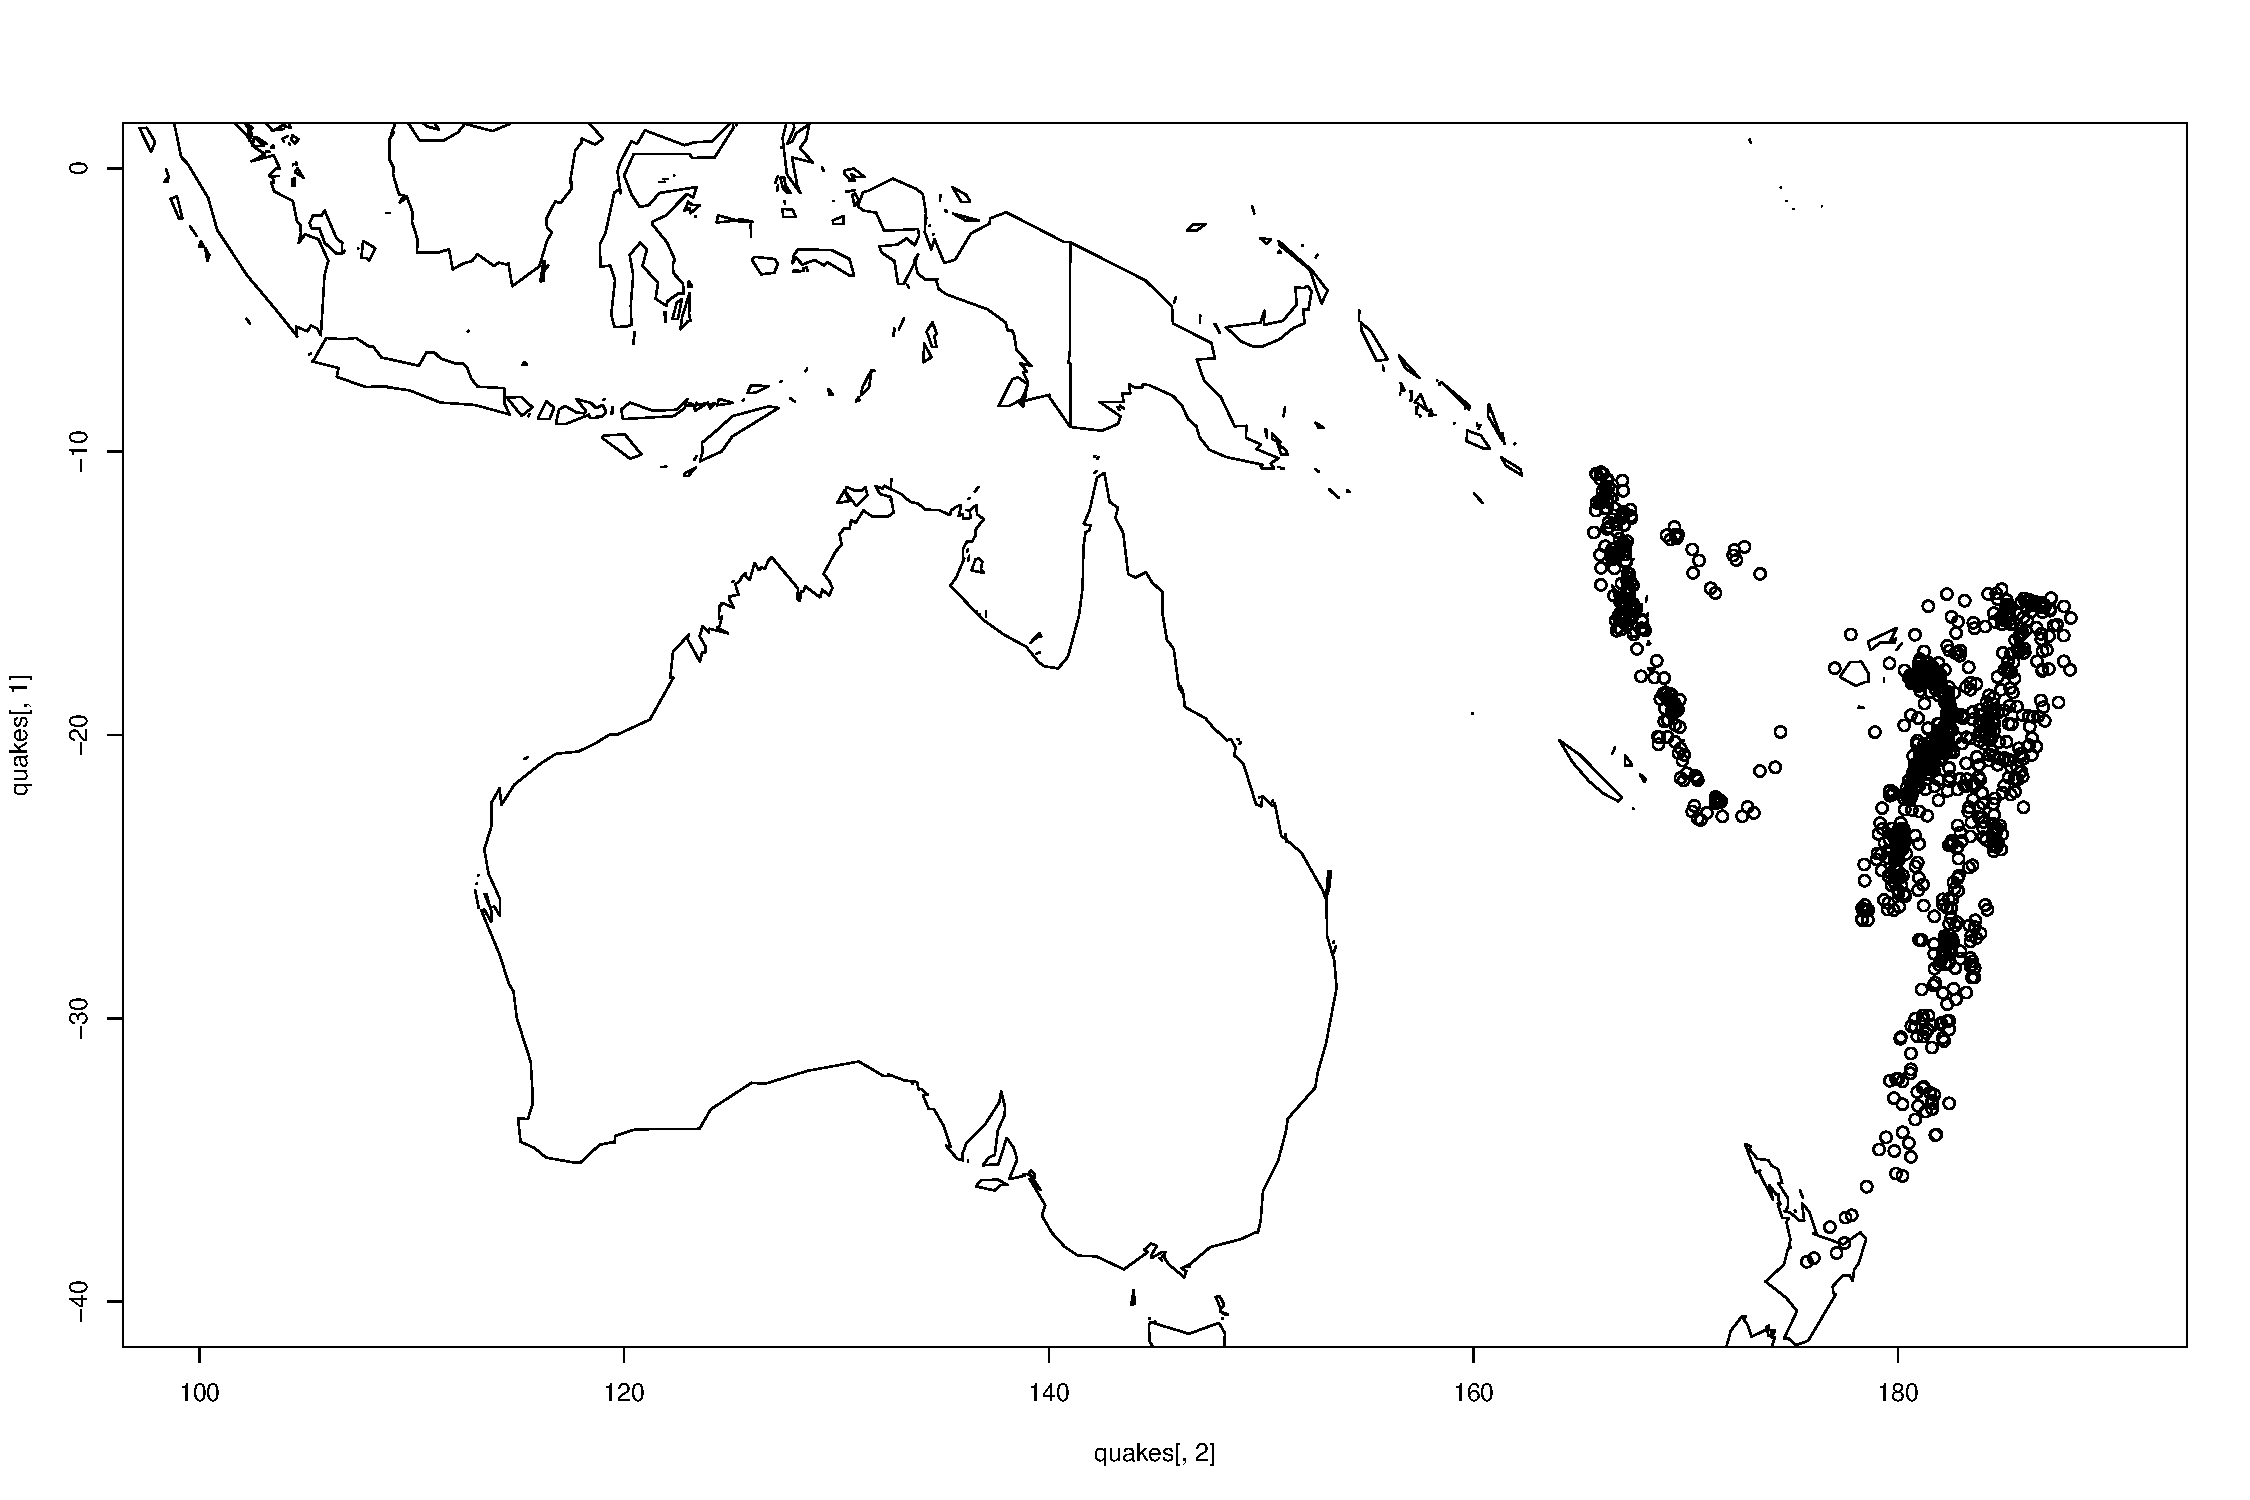
\includegraphics[width = 55mm]{images/Fuji.pdf}
\end{center}
\end{columns}
\end{frame}

%%%%%%%%%%%%%%%%%%%%%%%%%%%%%%%%%%%%%
\subsection{Projection Maps}
%%%%%%%%%%%%%%%%%%%%%%%%%%%%%%%%%%%%%

\begin{frame}[allowframebreaks, fragile]
\frametitle{Projection Maps}
  \framesubtitle{Map of Fiji Earthquakes Since 1964}

For a different perspective of a map, use  \ttfamily mapproject(): \normalfont 

\begin{lstlisting}
library(mapproj)
library(maps)
m <- map('world',plot=FALSE)
# Projection is Azimuthal with equal-area
map('world',proj='azequalarea',orient=c(longitude=0,latitude=180,rotation=0))
map.grid(m,col=2)
points(mapproject(list(y=quakes[which(quakes[, 4]>=6), 1],x=quakes[which(quakes[, 4]>=6), 2])),col="blue",pch="x",cex=2)
\end{lstlisting}

\newpage
       \begin{center}
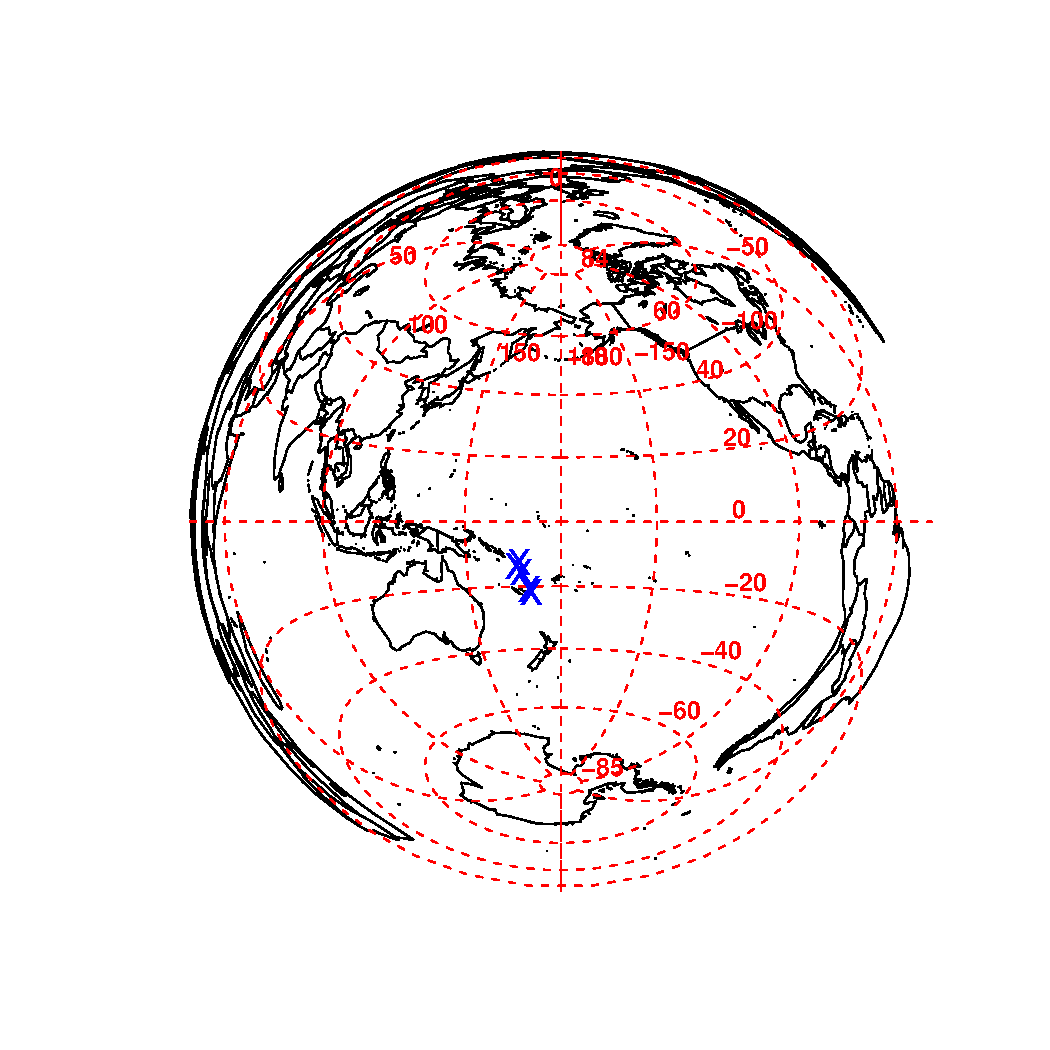
\includegraphics[width = 70mm]{images/Fuji2.pdf}
\end{center}

\end{frame}

%%%%%%%%%%%
\begin{frame}[fragile]
	\begin{alertblock}{Bonus Feature of the \ttfamily maps \normalfont package:}
		To determine in which part of the world the observations are (based on latitude and longitude), use \ttfamily map.where(): \normalfont
			\begin{lstlisting}		
				in.what.country<-map.where(database="world", quakes[, 2], quakes[, 1])
			\end{lstlisting}
		To determine which observations are in the ocean: \normalfont
			\begin{lstlisting}
				# Number of points in ocean after filtering:
				ind<-sum(is.na(in.what.country)); ind
				# Number of observations: 1000
				# Number in Ocean: 993
			\end{lstlisting}
	\end{alertblock}

\end{frame}

% ------------------------------------------------------------
% ------------------------------------------------------------
